\usepackage{gensymb}
\usepackage{listings}
\usepackage{hyperref}

\newenvironment{absolutelynopagebreak}
  {\par\nobreak\vfil\penalty0\vfilneg
   \vtop\bgroup}
  {\par\xdef\tpd{\the\prevdepth}\egroup
   \prevdepth=\tpd}
   


\begin{document}
%
% paper title
% can use linebreaks \\ within to get better formatting as desired
\title{Effects of VFD drive system on motor winding insulation}


% author names and affiliations
% use a multiple column layout for up to three different
% affiliations
%\author{
%\IEEEauthorblockN{David Kiss}
%\IEEEauthorblockA{School of Electrical and\\Computer Engineering\\
%Georgia Institute of Technology\\
%Atlanta, Georgia 30332--0250\\
%Email: http://www.michaelshell.org/contact.html}
%\and
%\IEEEauthorblockN{Homer Simpson}
%\IEEEauthorblockA{Twentieth Century Fox\\
%Springfield, USA\\
%Email: homer@thesimpsons.com}
%\and
%\IEEEauthorblockN{James Kirk\\ and Montgomery Scott}
%\IEEEauthorblockA{Starfleet Academy\\
%San Francisco, California 96678-2391\\
%Telephone: (800) 555--1212\\
%Fax: (888) 555--1212}}

% conference papers do not typically use \thanks and this command
% is locked out in conference mode. If really needed, such as for
% the acknowledgment of grants, issue a \IEEEoverridecommandlockouts
% after \documentclass

% for over three affiliations, or if they all won't fit within the width
% of the page, use this alternative format:
% 
%\author{\IEEEauthorblockN{Kiss Dávid}
%\IEEEauthorblockA{Budapesti Műszaki és Gazdaságtudományi Egyetem\\
%Automatizálási és Alklmazott Informatika Tanszék \\
%E-mail: david.kiss@aut.bme.hu;}
%}

\author{\IEEEauthorblockN{David Kiss}
\IEEEauthorblockA{Budapest University of Technologies and Economics\\
Department of Automation and Applied Electronics \\
E-mail: david.kiss@aut.bme.hu;}
}


% use for special paper notices
%\IEEEspecialpapernotice{(Invited Paper)}


% make the title area
\maketitle


\begin{abstract}
%\boldmath
Nowadays conventional electrical motors designs are facing the issue of the increasing number of variable frequency drives (VFDs). Motors fed with VFD systems had to withstand voltage stress with much higher voltage peaks, frequencies and slew rates than seen in grid powered motors. Due to the higher input frequency, the parasitic capacitance of the input cable and the inductance of the motor itself can cause resonance, with voltage spikes multiple times than the nominal voltage. Reflections due to impedance mismatches are also have to be taken account. The additional voltage stress can result in partial discharges (PD), faster insulation degradation, or even insulation breakdown. The presented paper will describe these effects in detail and provide a short introduction into the measures against the failures.
\end{abstract}
% IEEEtran.cls defaults to using nonbold math in the Abstract.
% This preserves the distinction between vectors and scalars. However,
% if the journal you are submitting to favors bold math in the abstract,
% then you can use LaTeX's standard command \boldmath at the very start
% of the abstract to achieve this. Many IEEE journals frown on math
% in the abstract anyway.

% Note that keywords are not normally used for peerreview papers.
\begin{IEEEkeywords}
Motor winding insulation, inverter, harmonics, PWM
\end{IEEEkeywords}


% For peer review papers, you can put extra information on the cover
% page as needed:
% \ifCLASSOPTIONpeerreview
% \begin{center} \bfseries EDICS Category: 3-BBND \end{center}
% \fi
%
% For peerreview papers, this IEEEtran command inserts a page break and
% creates the second title. It will be ignored for other modes.
\IEEEpeerreviewmaketitle


\section{Introduction}

In the world electrical energy usage, electrical drive systems are one of the biggest contributors. They are present from the few Watts to the Megawatt range. Focusing on the low voltage segment, DC motors were used in wide ranges due to the simplicity of their control. However with the progress of the semiconductor industry, VFD drives get more and more affordable even in the smallest segments. Three phase AC machines (both sinusoidal and trapezoidal field ones) gained their market share quickly. Because the lack of the brushes and the commutator, they are practically maintenance free, and more quiet. With modern drive controls they are precisely controllable, even in servo or high precision drives.

With the introduction of VFD systems, conventional electrical motor lifetimes are noticeably shorter. VFD drives applying a new type of stress on the motors, because of their operation principle. The output voltage has much higher frequency elements, the voltage slew rate can cause reflections on the motor cable, and harmonics and asymmetry can course current flow on he motor shaft and the bearings. 

\begin{figure}[h]
 \centerline{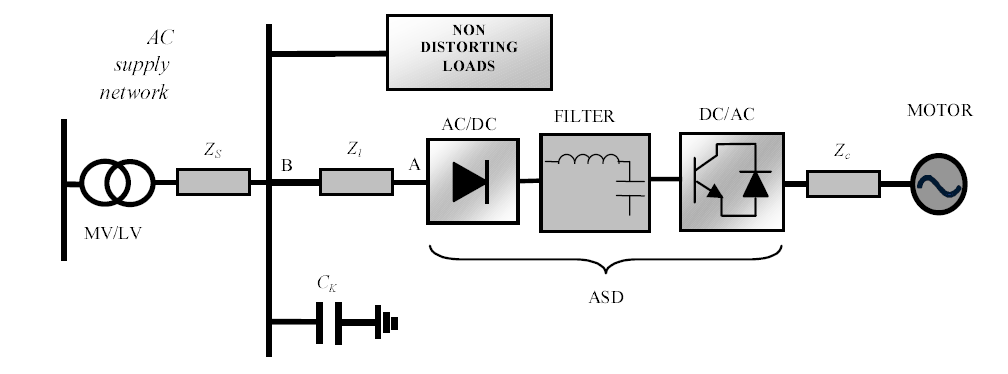
\includegraphics[width=.85\columnwidth]{.//figures/ac_plant.png}}
 \caption{Random and formed winding.}
 \label{fig:acplant}
\end{figure}

A average industrial drive system overview is presented on Figure \aref{fig:acplant}. Huge industrial facilities are usually have their own low voltage grid, or even middle voltage grid, depending on the used power. These subgrids are locally compensated for reactive power. There are other devices supplied by this grid, so EMC/EMI considerations are also have to be taken account. Because in most application, individual motor speed adjustments are necessary, Variable Frequency Drives are applied for the high power drives as well. This high power drives are operating with lower switching frequency, causing high amount of low order harmonics currents in the motors, which leads to additional thermal stress. Thermal degradation is also a limiting factor of the motors lifetime.


\subsection{Insulation in electrical machines}

Electrical motors are the devices which can convert electrical power to mechanical, based on electromagnetic principles. Therefore the largest part of the motor is built from electrically conductive materials. The point of the electrical insulation in electrical machine is to keep the electrical current in the desired conductors. The design goal with electrical machines is to achieve as high power density as possible both in volume and mass. In this approach insulation is not provide any value, however it is necessary to keep the machine functional. The conclusion is to keep the insulation as thin and as light as possible to provide space to magnetically and electrically active volumes, without compromising reliability.

Reliability means that these insulation systems are withstanding the normal operation stresses with high enough safety margin to overcome transients and expectable anomalies. The stresses on the motor insulations are present in multiple different manners. To overcome them, the insulator system should have the following properties.

\subsection*{Electrical stresses}
\begin{itemize}
	\item High breakdown voltage.
	\item Good long life performance .
	\item Low number of partial discharges (no voids in the material).
	\item Small leakage and creepage currents.
\end{itemize}

\subsection*{Thermal stresses}
\begin{itemize}
	\item Low degradation over time.
	\item Small deformation during thermal cycles .
	\item No delamination or disintegration.
\end{itemize}

\subsection*{Mechanical stresses}
\begin{itemize}
	\item High mechanical strength to sustain forces due to handling and mechanical forces under operation.
	\item Least reduction of mechanical strength within specified operating temperature and voltage.
\end{itemize}

These complex demands are presenting a challenging task to engineers, to the manufacturers, and for the insulation material as well. There are standards which defining and classifying insulator properties applied in electrical machines. These standards are the IEC 60085 and the IEC 60034-1.
A brief description of the insulating materials in use for different classes of insulation is given below to provide an introduction to the types of materials being used in the preparation of a particular class of insulation. The actual ingredients may be an improved version of these materials, in view of continuous researches and development in this field, to search out for still  better and more suitable materials.

\subsubsection*{Insulation Class A}
This includes organic fibrous materials on a cellulose base such as paper, pressboard, cotton, cotton cloth and natural silk etc., impregnated with lacquers or immersed in an insulating liquid. The impregnation or immersion ensures that the oxygen content of the air does not affect the insulating properties or enhance the thermal ageing of the insulating material. Typical materials in this class are varnished cloth and oil-impregnated paper.

\subsubsection*{Insulation Class E}
This includes wire enamels on a base of polyvinyl formal, polyurethane or epoxy resins as well as moulding powder plastics on phenol-formaldehyde and similar binders, with cellulose fillers, laminated plastics on paper and cotton cloth base, triacetate cellulose films, films and fibres of polyethylene terephthalate.

\subsubsection*{Insulation Class B}
This includes inorganic materials such as mica, glass fibre and asbestos etc., impregnated or glued together with varnishes or compositions comprising ordinary organic substances for heat resistance such as oil-modified synthetic resins, bitumen, shellac and Bakelite.

\subsubsection*{Insulation Class F}
This includes inorganic materials such as glass fibre or polyester and mica impregnated or glued together with epoxy, polyesterimide (polyamide or polyimide), polyurethane or other resins having superior thermal stability.

\subsubsection*{Insulation Class H}
This comprises composite materials on mica, glass fibre and asbestos bases, impregnated or glued together with silicone resins or silicone elastomer. These materials must not contain any organic fibrous materials such as paper or cloth backing, which is covered under class B and even F insulation systems.

The temperature limit of each class is presented in Table \ref{tab:temp}. The temperature values defined are assuming 20 years of working life.

\begin{table}[h]
\begin{tabular}{llll}
\hline
Class of insulation & Maximum attainable temperature\\ as in IEC 60085 & \multicolumn{2}{l}{Permissible operation temperature\\as in IEC 60034-1 by the resistance method} \\ \cline{3-4} 
                    &                                                & Up to 5 MW                                      & Above 5 MW                                     \\ \hline
                    & °C                                             & °C                                              & °C                                             \\
A                   & 105                                            & 100                                             & 100                                            \\
E                   & 120                                            & 115                                             & 110                                            \\
B                   & 130                                            & 120                                             & 120                                            \\
F                   & 155                                            & 145                                             & 145                                            \\
H                   & 180                                            & 165                                             & 165                                            \\ \hline
\end{tabular}
\caption{Insulation classes}
\label{tab:temp}
\end{table}
The development of the squirrel cage induction motor, with its associated insulation system,has generally been for sinusoidal supplies. Its design is well proven and inherently robust
leading to long reliable service with minimum maintenance.
One of the major reason behind motor failures is insulation aging and degradations. These effects are not caused by the VFD drive feeding, but it can be accelerated due the high frequency input. Over time, th insulation becomes more and more brittle, the thermal expansion cycles and the mechanical stress will cause small cracks. This small cracks are become larger and larger, pollution and moisture can reach to the conductor, and the insulation will be weaker and weaker, or starts disintegrating. The life expectancy of the insulation will also be affected by an excessive  operating temperature. It is halved for every 11∞C rise in temperature over its rated value and occurs when a machine is occasionally over-loaded. Sometimes the size of the machine may be only marginal when it was initially chosen and with the passage of time, it may be required to perform duties that are too arduous.
Practical life of insulation systems, and hence motor life, can be many years with ultimate failure likely to be through thermal and mechanical degradation of the insulating materials, not by
short-term direct electrical breakdown.

\subsection{Insulations systems}
\subsubsection{Steel lamination insulations}
The body of the electrical motor is laminated to prevent eddy currents. These laminates have to be insulated from each other to keep the eddy currents inside them. For small rating this is provided by oxidizing the surface of each plate on both side. For large ratings some resin layer is applied for one or both sides on the plates.

\subsubsection{Winding insulations}

Different manufacturers adopt to different practices of insulating the coil or the windings. Impregnation in a recommended insulating varnish, normally synthetic or epoxy, followed by baking (curing), in a temperature-controlled oven, at a specified temperature for a specific period.
For powerhouse insulation treatment the stator may be dipped in varnish for a minimum two to three times, each dipping being followed by backing. Sometimes one immersion of the entire stator and
two additional immersions of the overhangs followed by backing may also be sufficient.

\subsubsection*{Random winding}

The motor winding is constructed by wire, usually copper. If the winding is applied without any external formatting, it is called random winding. In this case the wires in one slot are not aligned in uniform manner, they filling up the space randomly, causing uneven distances, and air gaps between the wires. Increasing the risk of possible voids during impregnation.

\begin{figure}[h]
 \centerline{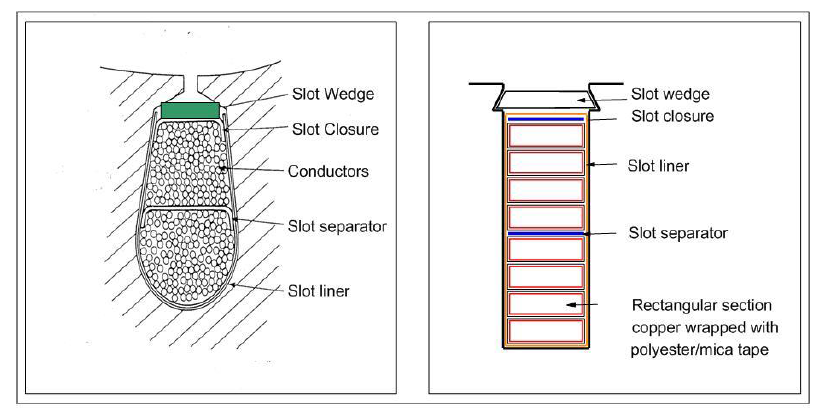
\includegraphics[width=.85\columnwidth]{.//figures/random_vs_formed.png}}
 \caption{Random and formed winding.}
 \label{fig:rnd vs formed}
\end{figure}

\subsubsection*{Formed winding}

For large motors, the practice is to wind the stator with formed coils (Figure 9.2). The coils are pre-formed and cured before insertion into the stator slots. They are insulated with resin-rich glass and mica paper tapes. The process of impregnation is therefore termed ‘resin-rich’ insulation. The completed formed wound stator is then heated to remove trapped moisture and finally impregnated in varnish class F or H as required. While vacuum pressure impregnation is the preferred method being more reliable, as noted below, other methods also providing satisfactory results and being economical are practiced by many manufacturers up to 1000 kW or so. The stator is then cured in an oven as described above. The process of insulation and curing conforms to powerhouse insulation requirements. This practice facilitates easy removal of an individual coil at site in case of a damage and replacement with a spare coil.

\begin{figure}[h]
 \centerline{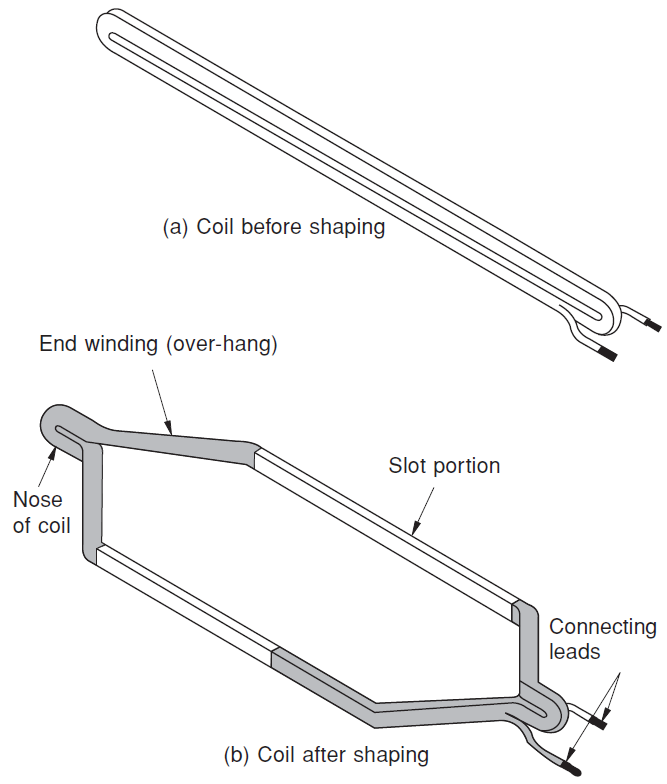
\includegraphics[width=.85\columnwidth]{.//figures/form_coil.png}}
 \caption{View of a formed coil.}
 \label{fig:form_coil}
\end{figure}


\section{VFD drive properties}

\section{Insulation failure mechanism}

\subsection{Overvoltage due reflections}

The PWM pulse rise-times are so short that their propagation along the motor cable to the motor can change the pulse shape and may produce a voltage overshoot. The cable can be considered as a transmission line, i.e. a long string of distributed series/parallel connected, inductor-capacitor sections as shown in Figure 3. For simplicity only one phase is represented.

At each pulse edge, the drive has to charge the inductance and capacitance of the cable, so a pulse of energy is delivered into the cable.
Transmission line theory shows that the pulse travels at a speed equal to 1/√𝐿𝐶 m/s, where L (Henries) and C (Farads) are the inductance and capacitance per meter, respectively. The velocity of propagation of a pulse in a typical PVC-insulated cable is about 1.7 x 108 m/s (i.e. in 100 ns the pulse travels only 17 m). It varies little over the variety of cable types in general use, since it is determined mainly by the permittivity of the internal insulating material.
The essential features of how a pulse propagates along the motor cable are illustrated in Figure 4 to Figure 7, and Figure 8 on the following pages.

Motor peak voltage is therefore a function of both cable length and rise time. For example, with 20 m of cable with a velocity of 1.7 x 108 m/s, any pulse with a rise-time less than 235 ns can
be expected to increase by nearly 100\%. Figure 9 shows some typical measured voltage waveforms (based on a 460 V test supply) which show this effect in practice. Even with 4 m of cable some overshoot is apparent. With 42 m the overshoot is virtually 100\%.

\subsection{Winding Voltage}
The voltage overshoot has little effect on the main motor insulation systems between phases and from phase to earth, which are designed to withstand large over voltages. However,
because of its short rise-time the voltage overshoot also stresses the insulation between turns, and especially between randomly touching conductors within a coil or between coil ends.
The front edge of the voltage pulse with its succession of voltage peaks (Figure 8) will travel around the motor winding as it does along the motor cable, with a measurable propagation
time. Figure 11 illustrates how this may result in a large proportion of the pulse appearing between turns, at random points within a coil or between coil ends. This effect progressively
decays to a uniform voltage distribution in subsequent coils due to high frequency inductive and capacitive losses.

Dependent on motor and winding parameters (e.g. motor rating, type of winding, number of turns, size of coil, turn propagation time etc) and the time between reflected peaks in the Page 13 of 29
incident terminal voltage, the voltage appearing between turns or randomly within a coil may briefly reach between 30\% and 90\% of the incident peak voltage.

Figure 12 shows the possible variations in first coil voltage plotted against the rise time of the incident peak voltage plotted against the rise time of the incident peak voltage at the motor
terminals.
With a sinusoidal supply voltage (uniformly distributed), the coil ends only experience a fraction of the phase voltage, as determined by the number of coils. With a variable speed drive
therefore, there can be a considerable increase in the voltage stress within a coil.

\subsections{Insualtion Breakdowns}
There are three suggested possibilities for insulation damage:-
 Breakdown between coil and stator core
Normally not a problem as slot liners are used
 Phase to phase failure - in the slots or end-windings
Normally not a problem as motors use inter-phase barriers (or are form-wound)
 Inter-turn failure between adjacent conductors in the stator winding
The most probable cause of failure due to the non-uniform distribution of voltage
along the stator windings, associated with the short rise times of the incident
voltage pulses as described in Section 2.With form wound motors, this is a less
significant problem because the turns are evenly distributed within the slot.
Depending upon the homogeneity of the stator winding materials and impregnation, there may
be voids in the impregnating resin, see Figure 19. It is in such voids that the failure mechanism
in the inter-turn insulation occurs. The failure mechanism is a complex phenomenon called
partial discharge (PD).
PD is a low energy discharge that occurs when both the following conditions apply:
 The peak value of the applied voltage is lower than the actual breakdown voltage of
the insulation system
 The local electric field intensity that is created in a void or cavity is sufficient to
exceed the breakdown strength in air (Partial Discharge Inception Voltage)

When subject to continuous partial discharges, the insulation system progressively degrades,
prematurely ageing the insulation material. The ageing process results from an erosion of the
insulation material, reducing its thickness at the discharge sites until its breakdown voltage
capability is reduced to below the level of the applied voltage peak, at this stage insulation
breakdown occurs.
Investigations, particularly at Dresden University [3] have produced relationships for model
insulation systems between the applied peak voltage, rise times, the probability of PD and the
insulation lifetime. The results are shown in Figure 20 for a reference temperature of 20°C with
a typical standard induction motor insulation system that is rated for operation with a nominal
supply voltage up to 500V a.c. on an inverter supply.
Figure 20 (a) which is based on the Dresden results, shows the cumulative number of pulses
(0.1 μs rise time, 5 μs duration) that the insulation should survive whilst Figure 20 (b) shows
the probability of PD occurring, both plotted against the pulse amplitude of the applied voltage.
PD inception voltage is influenced by temperature.

\section{Preventing insulation over-stress}

In applications where it is not feasible to employ motors which meet the withstand capability
achieved with standard or enhanced insulation given in Figure 21 curve A or B respectively,
some form of alternative solution is required.
Examples where these alternative solutions may be required include:
 Undefined motor characteristics
 Retrofit application of VSDs to ‘old’ motors
 Motors with inadequate pulse withstand capabilities
In the above cases, some form of motor terminal voltage modification technique is necessary.
These techniques essentially involve placing additional apparatus between the motor and the
inverter to limit the rate of rise of the pulse, reduce the reflection coefficient and thereby reduce
the peak voltage level. Some of the devices are also used to compensate for large capacitive
cable charging currents. These techniques may be summarised as follows:
 Output Reactors
 Output dv/dt Filters (sometimes known as dU/dt filters)
 Sinusoidal Filters
 Motor Termination Units
These solutions should be correctly matched to the application and the basic characteristics
are as described below.
In each case the effects of volt drop in the device on the final terminal voltage should be
established.

\section{Inverter rated motors}








\section{Summary}

A combination of fast switching semiconductors and ‘long’ motor cables can cause
peak voltages up to twice the DC link voltage (2.7 times the supply voltage) due to
transmission line effects. In extreme cases, this high peak voltage and the uneven
voltage distribution in the motor windings can cause a low energy partial discharge
between turns of the first coil. Partial discharge can cause premature ageing effects of
the winding insulation system until failure occurs.
 By selecting the correct motor, or by the use of appropriate preventative measures,
damaging partial discharge can be avoided, thereby ensuring the maximum motor life
is achieved.



%\begin{figure}[h]
%\centering
%\includegraphics[width=0.9\columnwidth]{figures/foster.png}
%% where an .eps filename suffix will be assumed under latex, 
%% and a .pdf suffix will be assumed for pdflatex; or what has been declared
%% via \DeclareGraphicsExtensions.
%\caption{The Foster thermal model}
%\label{fig:foster}
%\end{figure}



\


% needed in second column of first page if using \IEEEpubid
%\IEEEpubidadjcol

% An example of a floating figure using the graphicx package.
% Note that \label must occur AFTER (or within) \caption.
% For figures, \caption should occur after the \includegraphics.
% Note that IEEEtran v1.7 and later has special internal code that
% is designed to preserve the operation of \label within \caption
% even when the captionsoff option is in effect. However, because
% of issues like this, it may be the safest practice to put all your
% \label just after \caption rather than within \caption{}.homahazkezeles@gmail.comhomahazkezeles@gmail.com
% Reminder: the "draftcls" or "draftclsnofoot", not "draft", class
% option should be used if it is desired that the figures are to be
% displayed while in draft mode.
%
%\begin{figure}[!t]
%\centering
%\includegraphics[width=2.5in]{myfigure}
% where an .eps filename suffix will be assumed under latex, 
% and a .pdf suffix will be assumed for pdflatex; or what has been declared
% via \DeclareGraphicsExtensions.
%\caption{Simulation Results}
%\label{fig_sim}
%\end{figure}

% Note that IEEE typically puts floats only at the top, even when this
% results in a large percentage of a column being occupied by floats.


% An example of a double column floating figure using two subfigures.
% (The subfig.sty package must be loaded for this to work.)
% The subfigure \label commands are set within each subfloat command, the
% \label for the overall figure must come after \caption.
% \hfil must be used as a separator to get equal spacing.
% The subfigure.sty package works much the same way, except \subfigure is
% used instead of \subfloat.
%
%\begin{figure*}[!t]
%\centerline{\subfloat[Case I]\includegraphics[width=2.5in]{subfigcase1}%
%\label{fig_first_case}}
%\hfil
%\subfloat[Case II]{\includegraphics[width=2.5in]{subfigcase2}%
%\label{fig_second_case}}}
%\caption{Simulation results}
%\label{fig_sim}
%\end{figure*}
%
% Note that often IEEE papers with subfigures do not employ subfigure
% captions (using the optional argument to \subfloat), but instead will
% reference/describe all of them (a), (b), etc., within the main caption.


% An example of a floating table. Note that, for IEEE style tables, the 
% \caption command should come BEFORE the table. Table text will default to
% \footnotesize as IEEE normally uses this smaller font for tables.
% The \label must come after \caption as always.
%
%\begin{table}[!t]
%% increase table row spacing, adjust to taste
%\renewcommand{\arraystretch}{1.3}
% if using array.sty, it might be a good idea to tweak the value of
% \extrarowheight as needed to properly center the text within the cells
%\caption{An Example of a Table}
%\label{table_example}
%\centering
%% Some packages, such as MDW tools, offer better commands for making tables
%% than the plain LaTeX2e tabular which is used here.
%\begin{tabular}{|c||c|}
%\hline
%One & Two\\
%\hline
%Three & Four\\
%\hline
%\end{tabular}
%\end{table}


% Note that IEEE does not put floats in the very first column - or typically
% anywhere on the first page for that matter. Also, in-text middle ("here")
% positioning is not used. Most IEEE journals use top floats exclusively.
% Note that, LaTeX2e, unlike IEEE journals, places footnotes above bottom
% floats. This can be corrected via the \fnbelowfloat command of the
% stfloats package.




% if have a single appendix:
%\appendix[Proof of the Zonklar Equations]
% or
%\appendix  % for no appendix heading
% do not use \section anymore after \appendix, only \section*
% is possibly needed

% use appendices with more than one appendix
% then use \section to start each appendix
% you must declare a \section before using any
% \subsection or using \label (\appendices by itself
% starts a section numbered zero.)
%





% Can use something like this to put references on a page
% by themselves when using endfloat and the captionsoff option.
\ifCLASSOPTIONcaptionsoff
  \newpage
\fi



% trigger a \newpage just before the given reference
% number - used to balance the columns on the last page
% adjust value as needed - may need to be readjusted if
% the document is modified later
%\IEEEtriggeratref{8}
% The "triggered" command can be changed if desired:
%\IEEEtriggercmd{\enlargethispage{-5in}}

% references section

% can use a bibliography generated by BibTeX as a .bbl file
% BibTeX documentation can be easily obtained at:
% http://www.ctan.org/tex-archive/biblio/bibtex/contrib/doc/
% The IEEEtran BibTeX style support page is at:
% http://www.michaelshell.org/tex/ieeetran/bibtex/
%\bibliographystyle{IEEEtran}
% argument is your BibTeX string definitions and bibliography database(s)
%\bibliography{IEEEabrv,../bib/paper}
%
% <OR> manually copy in the resultant .bbl file
% set second argument of \begin to the number of references
% (used to reserve space for the reference number labels box)
\begin{thebibliography}{1}


\bibitem{uni:hvlabor}
Energy density - Wikipedia article, \\
  \url{https://en.wikipedia.org/wiki/Energy_density#Energy_densities_of_common_energy_storage_materials}, \\Utolsó megtekintés: 2018.04.02.
  

\bibitem{article:char}
Ronen Hareuveny, Madhuri Sudan, Malka N. Halgamuge, Yoav Yaffe, Yuval Tzabari, Daniel Namir and Leeka Kheifets, Characterization of Extremely Low Frequency Magnetic Fields from Diesel, Gasoline and Hybrid Cars under Controlled Conditions \hskip 1em plus
  0.5em minus 0.4em\relax International Journal of Environmental Research and Public Health, 2015.
  
\bibitem{article:magnetic}
DAndrea Vassilev, Alain Ferber, Christof Wehrmann, Olivier Pinaud, Meinhard Schilling,
and Alastair R. Ruddle Magnetic Field Exposure Assessment
in Electric Vehicles \hskip 1em plus
  0.5em minus 0.4em\relax IEEE TRANSACTIONS ON ELECTROMAGNETIC COMPATIBILITY, 2015.
  

  
\bibitem{article:passanger}
Pablo Moreno-Torres Concha, Pablo Velez, Marcos Lafoz, and Jaime R. Arribas, Passenger Exposure to Magnetic Fields due to the Batteries of an Electric Vehicle, \hskip 1em plus
  0.5em minus 0.4em\relax IEEE TRANSACTIONS ON VEHICULAR TECHNOLOGY, 2016.

\bibitem{article:wireless}
Sangwook Park, Evaluation of Electromagnetic Exposure During 85 kHz Wireless Power Transfer for Electric Vehicles, \hskip 1em plus
  0.5em minus 0.4em\relax IEEE TRANSACTIONS ON MAGNETICS, 2018.

\bibitem{artice:emf}
Richard A. Tell1, and Robert Kavet, ELECTRIC AND MAGNETIC FIELDS <100 KHZ IN ELECTRIC AND GASOLINE-POWEREDVEHICLES, \hskip 1em plus
  0.5em minus 0.4em\relax Radiation Protection Dosimetry, Vol. 172, No. 4, pp. 541–546, 2016.
  
  \bibitem{artice:icnrip1}
ICNIRP,Guidelines on limits for exposure to static magnetic fields,, \hskip 1em plus
  0.5em minus 0.4em\relax Health Phys., vol. 96, no. 4, pp. 504–514, Apr. 2009.



\end{thebibliography}

% biography section
% 
% If you have an EPS/PDF photo (graphicx package needed) extra braces are
% needed around the contents of the optional argument to biography to prevent
% the LaTeX parser from getting confused when it sees the complicated
% \includegraphics command within an optional argument. (You could create
% your own custom macro containing the \includegraphics command to make things
% simpler here.)
%\begin{biography}[{\includegraphics[width=1in,height=1.25in,clip,keepaspectratio]{mshell}}]{Michael Shell}
% or if you just want to reserve a space for a photo:

\begin{IEEEbiography}[{\includegraphics[width=1in,height=1.25in,clip,keepaspectratio]{picture}}]{John Doe}
\blindtext



\end{IEEEbiography}

% You can push biographies down or up by placing
% a \vfill before or after them. The appropriate
% use of \vfill depends on what kind of text is
% on the last page and whether or not the columns
% are being equalized.

%\vfill

% Can be used to pull up biographies so that the bottom of the last one
% is flush with the other column.
%\enlargethispage{-5in}




% that's all folks
\end{document}


